\documentclass[tikz]{standalone}
\usepackage{amsmath}

\begin{document}

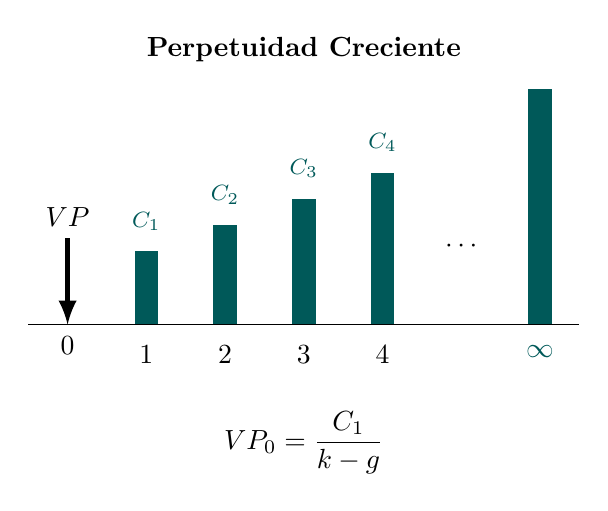
\begin{tikzpicture}
	\foreach \n in {1,...,4} 
	\draw [teal!70!black, line width = 3mm] 
	(\n,0) node [below] {\color{black}\(\n\)} 
	-- ++(0,0.6+\n/3) node [above] {\footnotesize \(C_\n\)};
	\draw [teal!70!black, line width = 3mm] 
	(6,0) node [below] {\(\infty\)} --++ (0,3);
	\node at (5,1) {\(\cdots\)};
	\draw [-latex, line width=0.7mm] 
	(0,1.1) node [above] {\(VP\)} -- (0,0) node [below] {\(0\)};
	\node at (3,3.5) {\textbf{Perpetuidad Creciente}};
	\node at (3,-1.5) {\(VP_0 = \dfrac{C_1}{k-g}\)};
	\draw (-0.5,0) -- (6.5,0);
\end{tikzpicture}

\end{document}
